\chapter{Introduction} 
\label{ch:intro}

\previouslypublished{Sections of this chapter have been previously published in \bibentry{Wilkins:2012ii}.}

\section{Physical Oceanography of the Southern Ocean}

The \ac{SO} is large (\textapprox{}36,000,000 km\textsuperscript{2}), oceanographically complex and an important part of the world's hydro- and biospheres.
It drives global \ac{THC}: \ac{AABW} formed off the Antarctic Coast is the major source of the World Ocean's \ac{BW} \cite{Jacobs:2004hv}, the sinking of which is one of two major engines for the \ac{THC} ``global conveyor belt'' (the other being \ac{BW} formation in the North Atlantic).
The \ac{SO} also supports a large fraction of global marine primary production: the upwelling of \ac{CDW} south of the \ac{PF} returns nutrients transported to the deep ocean by sinking particulate matter \cite{Rath:1998wm} to the surface.

These important functions are closely linked to the \ac{SO}'s unique oceanography.
Like the Arctic Ocean, the \ac{SO} is circumpolar, entailing physical features such as low surface water temperatures, strong seasonal cycles in temperature and solar irradiation, the seasonal formation of sea ice and exposure to surface sheer forces from strong high-latitude winds.
Unlike the Arctic Ocean, however, the \ac{SO} has broad interfaces with the tropical oceans and circumpolar circulation uninterrupted by any major land mass, and in Antarctic coastal waters experiences powerful katabatic winds off the Antarctic ice cap.
These properties shape the \ac{SO}'s unique physical oceanography.

\subsection{Fronts and zones}
\begin{figure}
  \centering
  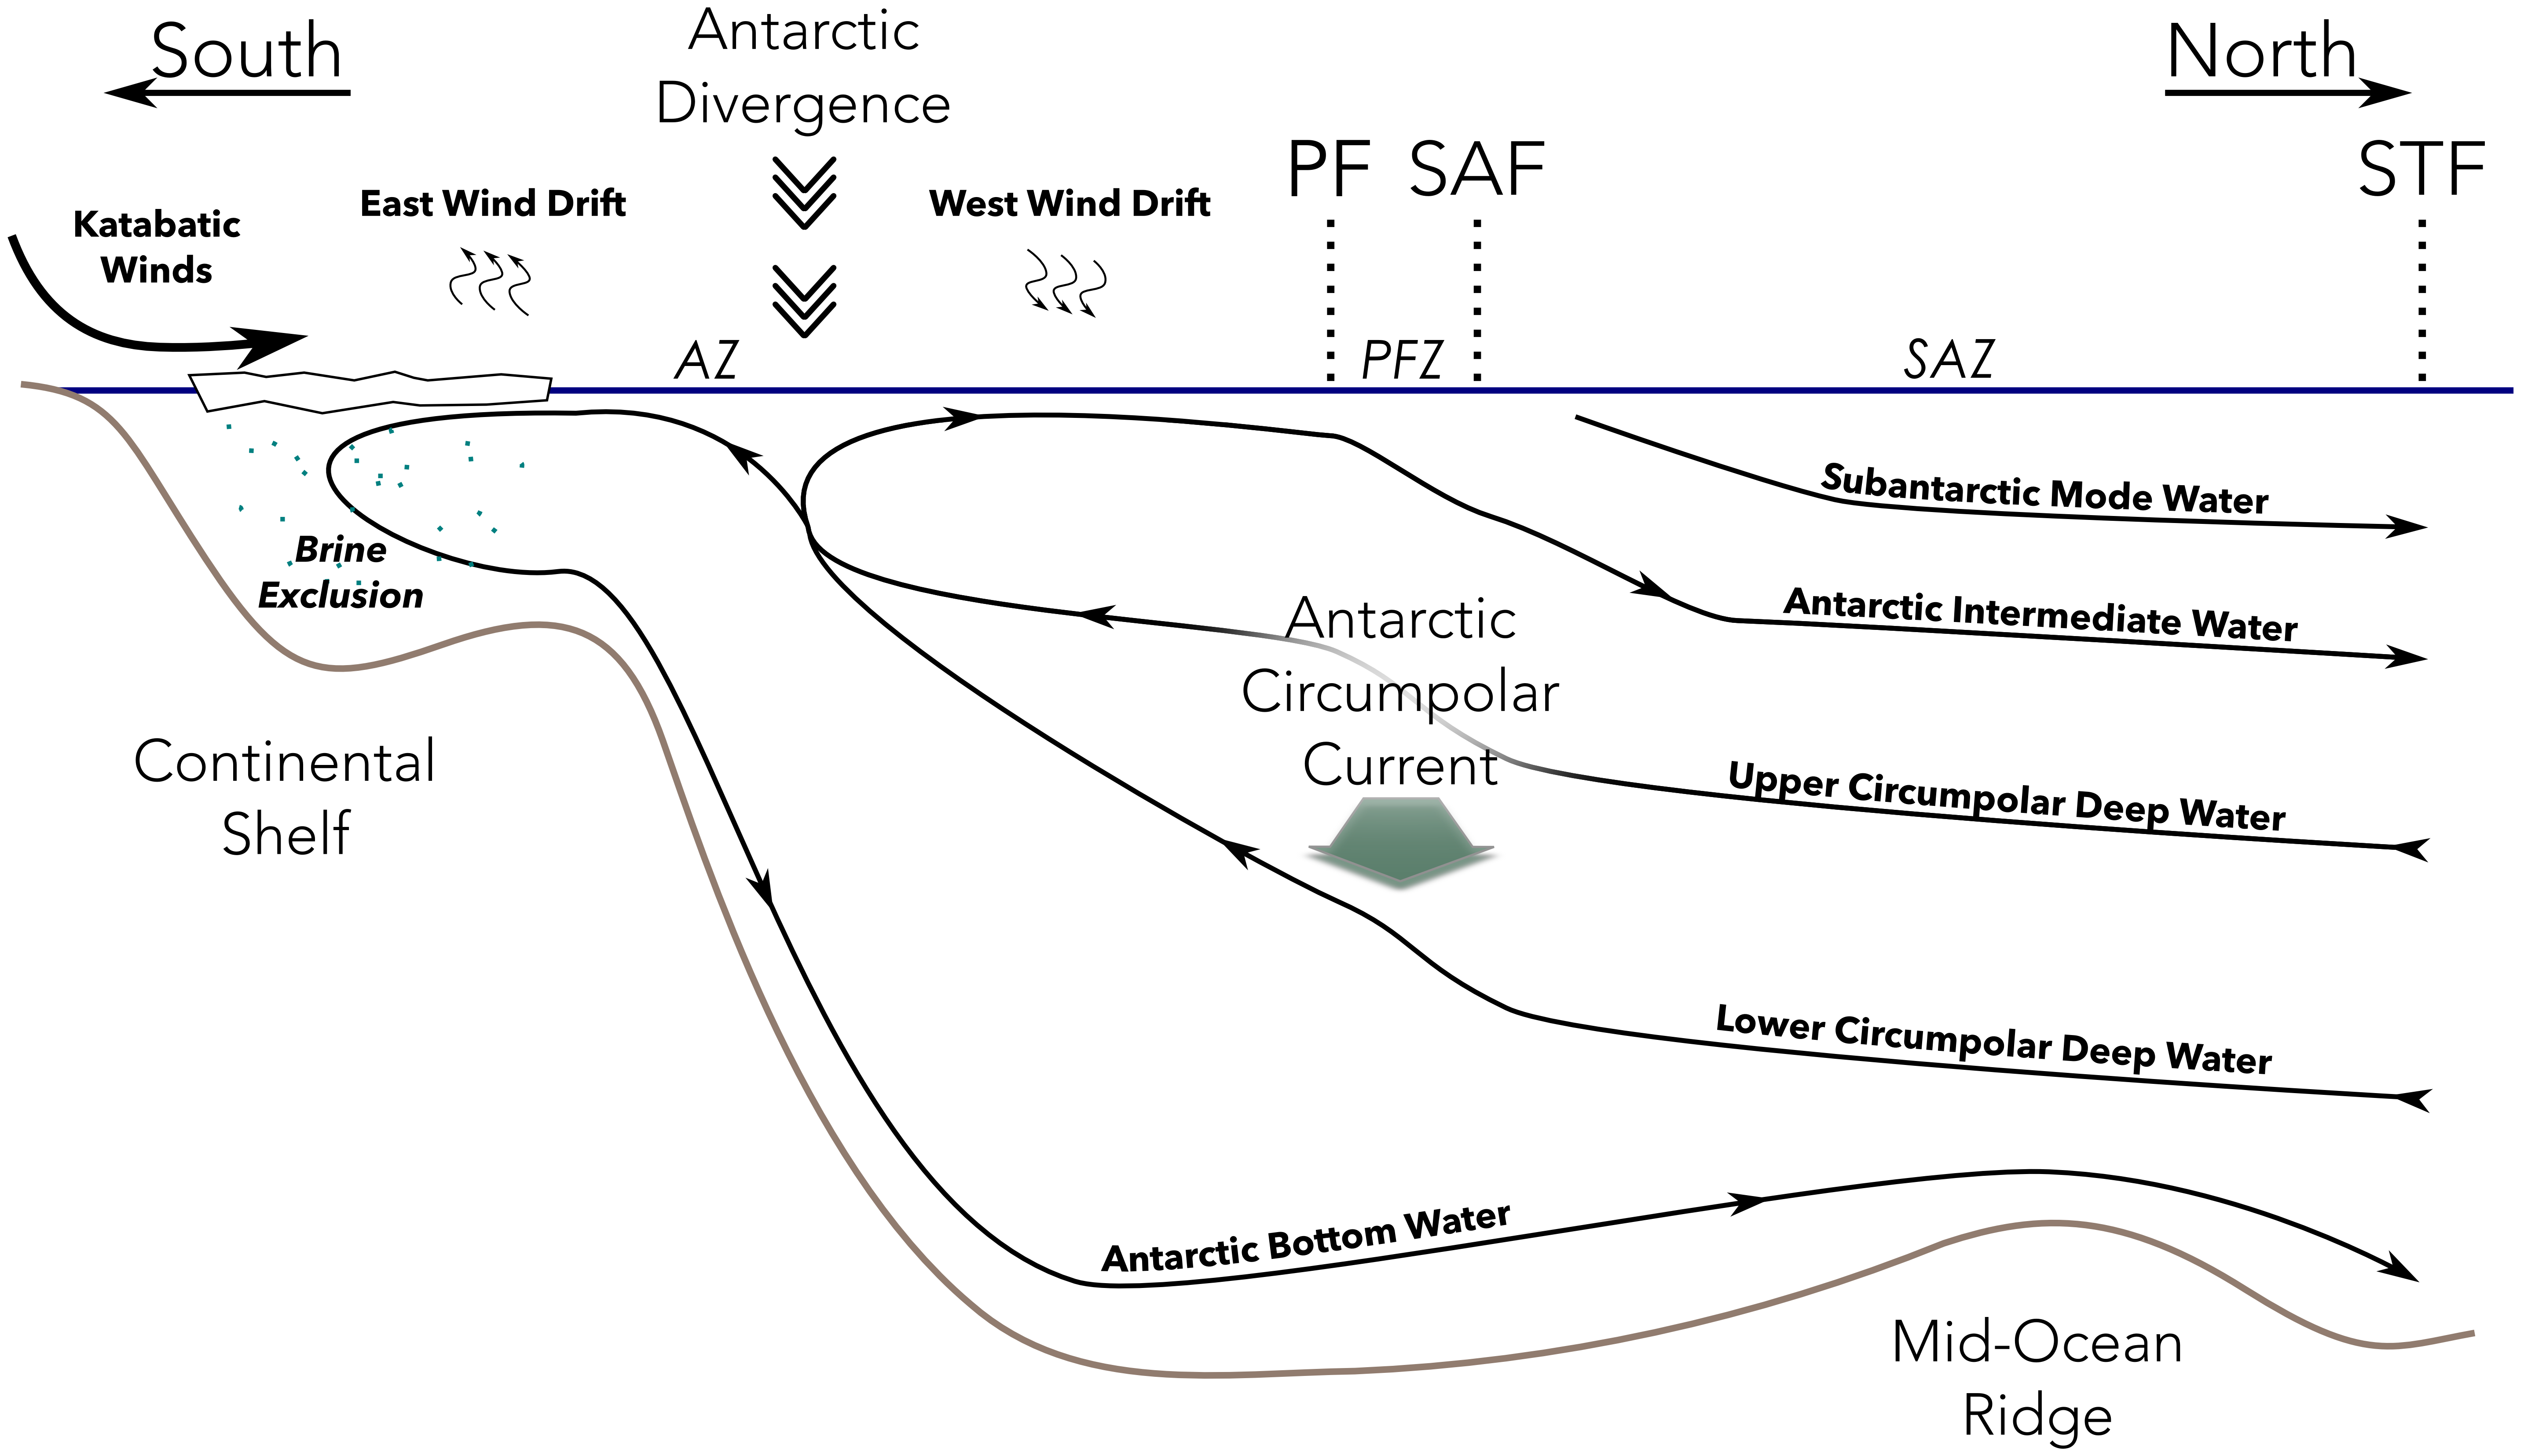
\includegraphics[width=\textwidth]{../introduction/oceanographymap.png}
  \caption[Major fronts and water masses of the Southern Ocean]{North--South cross-section of the Southern Ocean, showing major fronts and water masses.
  This map is schematic only and not to scale.
  Acronyms are as follows: Subtropical Front (STF); Subantarctic Zone (SAF); Subantarctic Front (SAF); Polar Frontal Zone (PFZ); Polar Front (PF); Antarctic Zone (AZ).}
  \label{fig:oceanographymap}
\end{figure}

Definitions of the \ac{SO}'s extent vary.
Features commonly used to define its northern boundary include the 60\textsuperscript{th} parallel south and the \ac{AC}, while most Australian cartographic and governmental bodies consider the \ac{SO} to begin at Australia's southern coastline, or approximately the 45\textsuperscript{th} parallel south.
The Australian definition will be used in this thesis.

The surface of the \ac{SO} is composed of several distinct zones, separated by circumpolar fronts \figref{fig:oceanographymap}.
Step transitions in the temperature and density of surface waters define the locations and extent of these fronts \cite{Sokolov:2002tc,Orsi:1995va}.
The northernmost front is the \ac{STF}, which lies at \textapprox{}40--45\textdegree{} S, separating the \ac{SAZ} from the warmer and saltier tropical oceans to its north \cite{Sokolov:2002tc}.
Across the \ac{STF}, potential temperature at 150 m depth decreases from \textgreater{} 12 to \textless{} 10 \textdegree{}C.

Moving southwards, the southern extent of the \ac{SAZ} is defined by the \ac{SAF}.
The \ac{SAF} is the northernmost and primary current core of the multiply-branched \ac{ACC} \cite{Sokolov:2009wp}, and its position is thus defined by that of the \ac{ACC} which varies considerably with longitude \cite{Moore:1999to}.
As with the \ac{STF}, there is a drop in potential temperature of 2--4 \textdegree{}C across the front \cite{Sokolov:2002tc}.
The \ac{SAF} also marks the northern boundary of the \ac{PFZ}, where the \ac{SAZ} and colder \ac{AZ} waters meet and mix.
Although both the \ac{SAF} and \ac{PF} represent large step changes in surface characteristics, the \ac{PFZ} itself is relatively constant \cite{WhitworthIII:1987ky}.
This zone, and particularly its bounding fronts, are regions of high primary productivity \citep[e.g.][]{Laubscher:1993hu,Abell:2005ji}.

The southern boundary of the \ac{PFZ} is the \ac{PF}, also a current core of the \ac{ACC}, and associated with a potential temperature drop of \textapprox{}1--1.5 \textdegree{}C \cite{Moore:1999to}.
The waters south of the \ac{PF} constitute the \ac{AZ}, the southernmost and coldest (\textless{} 2 \textdegree{}C, \citet{Sokolov:2002tc}) major zone.
The \ac{AZ} can be further subdivided by several minor features, including the \ac{SACCF} and \ac{SB}, both weaker southern branches of the \ac{ACC}.
However, these do not represent significant step transitions in physical properties.

\subsection{Water masses and circulation}

In addition to these surface features, the \ac{SO} comprises several distinct water masses \figref{fig:oceanographymap}, the circulation of which forms a major component of global \ac{THC}.
The most extensive of these is \ac{CDW}, which consists of two layers.
The \ac{UCDW}, characterised by a nutrient maximum and oxygen minimum, originates in the western Indian and south-eastern Pacific oceans \cite{Orsi:1995va}.
The \ac{LCDW}, characterised by a salinity maximum, originates as sinking \ac{NADW} \cite{WhitworthIII:1987ky}.
Both layers of \ac{CDW} shoal southwards across the \ac{ACC}.

South of the \ac{PF} is the Antarctic Divergence, a region of transition between dominant easterly and westerly winds.
As a consequence of Ekman flow generated by these winds, surface currents are divergent, with those to the north driven further northwards by the westerlies (the West Wind Drift) while those to the south are forced southwards by the easterlies (the East Wind Drift) \cite{Foldvik:1988gp}.
This generates a region of upwelling, where the \ac{UCDW} meet and interact with the upper ocean layers and atmosphere.

Between the divergence and the \ac{PF}, the surface layer (\textapprox{}100--300 m depth) consists of \ac{ASW}, which is colder, less saline and better ventilated (i.e.\ more oxygenated) than the \ac{CDW}.
Driven by Ekman transport in the West Wind Drift, the \ac{ASW} moves northwards towards the \ac{PF}, with isopycnals (surfaces of constant potential density) sloping gently downwards towards the north.
At the \ac{PF}, the \ac{ASW} sinks rapidly to form the \ac{AAIW} (\textapprox{}500--1500 m depth), a layer of low-salinity water which underlies \ac{SAZ} and, moving northwards, contributes to the intermediate water of the subtropical oceans \cite{Foldvik:1988gp}.
(Note that both the \ac{SAF} and \ac{PF} can be defined as the locations where the temperature minimum associated with \ac{AAIW} rapidly decreases in depth \cite{WhitworthIII:1987ky}.)
Overlying the \ac{AAIW} in the \ac{SAZ} is the \ac{SAMW}, which forms the surface layer north of the \ac{SAF} \cite{Speer:2000th}.
Although the \ac{SAF} is nominally the southern boundary of the \ac{SAMW}, the surface discontinuity may sometimes occur several degrees to the south of the sub-surface front \citep[e.g.][]{Deacon:1982ce,Orsi:1995va}

Surface and \ac{CDW} waters south of the Antarctic Divergence do not move northwards to form \ac{AAIW}, but instead are driven southwards by the East Wind Drift.
The region between the Antarctic Divergence and the coast is the site of dense, cold \ac{AABW} formation.
Katabatic winds from the Antarctic continent form polynyas and cool the surface waters, while brine exclusion during sea ice formation increases the waters' density.
This newly formed cold and dense \ac{AABW} sinks rapidly and flows down the continental shelf and margin to form an abyssal layer beneath the entire \ac{SO} \cite{Orsi:1999hz,Foldvik:1988gp}.
\ac{AABW} formation does not occur along the entire continental margin; rather, it is concentrated in the Weddell and Ross seas, and to a lesser extent the D'Urville sea off the Ad\'{e}lie Land coast.
\ac{AABW} is a major source of abyssal water to the World Ocean, and its formation drives global \ac{THC}.
Because \ac{AABW} is ventilated in the \ac{SO} before sinking rapidly, \ac{AABW} is relatively enriched in oxygen compared to other deep layers of the World Ocean, which are oxygen-depleted due to the heterotrophic oxidation of sinking organic matter.

\subsection{Effect of climate change}

Anthropogenic climate change is having a significant effect on the \ac{ACC} and the water masses it defines.
Changes in the \ac{SAM}, a regular pattern of Southern Hemisphere atmospheric circulation characteristics, are leading to an intensification of the westerly winds \cite{Thompson:2002ic} which drive the \ac{ACC}.
As a consequence of this and other climate change-related effects, the mean annual path of the \ac{ACC} and its associated fronts and isopycnals has moved \textapprox{}50 km southwards since the 1950s \cite{Gille:2002fr}.
Waters on the poleward side of the \ac{ACC} have become warmer and more saline, while those to the north cooler and fresher \cite{Boning:2008il}.
The \ac{ACC} itself is warming and freshening \cite{Boning:2008il}, from the surface to 900 m depth \cite{Aoki:2003fo}.

\citet{Fyfe:2005vp}, using a wind-driven model of the southward shift of the \ac{ACC}, predicted that with conservative assumptions about future anthropogenic greenhouse gas emissions (\ac{IPCC} A2 and B2 scenarios), the \ac{ACC} can be expected to move \textapprox{}1.4\textdegree{} southwards by the year 2100.
They note that this is equivalent to reducing the volume of the \ac{SO} south of the \ac{ACC} by about $16 \times{} 10^{6}$ \ce{km^{3}}, or approximately the volume of the Arctic Ocean.

Aside from the oceanographic effects, these changes can be expected to effect the biology of the \ac{SO}.
In particular, even neglecting the changes in temperature and salinity of the water masses defined by the \ac{ACC}, the southward migration of the \ac{ACC} and concomitant change in the relative volumes (and surface areas) of the water masses it defines are a significant change in the size of the microbial habitats these masses represent.
Predicting the effects this will have on \ac{SO} ecosystems and ecosystem functions requires an understanding of the microbial ecology of the \ac{SO}, and its biogeography relative to the \ac{ACC} and its associate fronts and water masses.
The following section gives an overview of the current state of knowledge.

\section{Microbial ecology of the Southern Ocean}

TODO
  - Microbes perform key ecosystem functions
  - Microbes are partitioned by fronts/zones (summarise here, more detail is in individual divisions)
  - Focus only on Picoplankton (but add gloss on eukarya?)
  - Focus only on molecular studies

\subsection{Bacteria}

\subsubsection{Alphaproteobacteria}

\subsubsubsection{Roseobacter clade}

The Roseobacter clade is an abundant and ecologically significant group of marine bacteria, found at high (> 15\%) abundance in most marine surface environments \citep[][and references therein]{Buchan:2005hd}.
Unlike some other major proteobacterial groups that are strongly associated with a particular ecological niche (e.g.\ the SAR11 clade), roseobacters have diverse metabolic abilities, with members capable of (for example) aerobic anoxygenic phototrophy \cite{Biebl:2005fp,Beja:2002gt}, degradation of \ac{DMSP} by at least two pathways \cite{Miller:2004jz,Moran:2003cwa}, carbon monoxide oxidation \cite{King:2003kc} and heterotrophic utilisation of a broad range of substrates \citep[reviewed in][]{Brinkhoff:2008do}.
Roseobacters are found in the planktonic fraction as well as in commensal association with phytoplankton and metazoans \citep[reviewed in][]{Buchan:2005hd}.

Several 16S rDNA-based studies have identified the \ac{RCA} subgroup as ubiquitous and abundant in \ac{SO} surface waters and to a depth of at least 2200 m, composing \textapprox{}10--30\% of surface bacteria (and the majority of roseobacters) in the Subantarctic and Antarctic zones \cite{Giebel:2009hr,Murray:2007db,Ghiglione:2011ee} and a major fraction of the population in coastal waters \cite{Murray:2007db,Koh:2011ij}.
Two major \ac{RCA} phylotypes appear to be present in the \ac{SO} and form the majority of the Roseobacter population.
The phylotypes are strictly segregated by the \ac{PF}, coexisting only within the \ac{PFZ} \cite{Selje:2004ka,Giebel:2009hr} where they may outnumber even the SAR11 clade.
There is some evidence that the \ac{AZ} \ac{RCA} phylotype originates from the North Atlantic; \citet{Giebel:2009hr} noted \ac{CDW} at 2200 m in the \ac{SZ} had an identical temperature-salinity signature to \ac{NADW}.
\ac{NADW} is formed by the sinking of dense, saline waters from the surface north Atlantic, and is transported to the \ac{SO} via global thermohaline circulation to become \ac{CDW} \cite{Callahan:1972tk}.
Consistent with the upwelling of \ac{CDW} in the \ac{AZ} south of the \ac{PF}, \citep{Selje:2004ka} reported in a global study of \ac{RCA} 16S rDNA gene fragments that the surface phylotype south of the \ac{PF} was identical to one found in the Arctic Ocean, while differing by 3 bp from that north of the \ac{PF}.

Little is known about the functional capabilities of \ac{RCA} as only two isolated representatives have been described to date.
\citep{Giebel:2010bsa} isolated \candidatus{Planktomarina temperata} from the North Sea, where it was the dominant phylotype.
The authors' identification of the pufM gene encoding a bacteriochlorophyll a subunit suggests at least this member of the \ac{RCA} is capable of performing aerobic anoxygenic photosynthesis, a function of potentially large ecological significance.
\citet{Mayali:2008eb} isolated an apparently heterotrophic \ac{RCA} member from subtropical waters, and found \emph{in vitro} evidence that they colonised and increased mortality in blooming dinoflagellates, but did not investigate photosynthetic potential.

Roseobacters, and particularly the \ac{RCA}, have been strongly associated with phytoplankton blooms in the \ac{SO}.
Two separate 16S rDNA-based studies of a naturally fertilised bloom in the Kerguelen islands region \cite{West:2008kc,Obernosterer:2011df} found that \ac{RCA} and the Roseobacter NAC11-7 and NAC11-6 clusters were dominant bacterial \acp{OTU} in the bloom patch, suggesting they play a role in heterotrophic degradation of bloom products.
Unlike the other clusters, however, \ac{RCA} representatives were also relatively abundant and metabolically active outside of the patch.
Both \citet{Giebel:2009hr} and \citet{Obernosterer:2011df} found that in \ac{SO} vertical profiles \ac{RCA} abundances often peaked at the deep chlorophyll maximum, again suggesting an association with phytoplankton.

\ac{RCA} abundance may follow a seasonal cycle in the \ac{SO}.
\citet{Giebel:2009hr} found that \ac{RCA} phylotypes were at maximum 8\% of all bacterial 16S rDNA genes during winter but up to 36\% in the coastal current and Weddell sea during autumn, while \citet{Ghiglione:2011ee} found the proportion to peak in January in coastal waters off the Antarctic Peninsula and in February off the Kerguelen islands. 

A metagenomic study of \ac{SO} waters off West Antarctica found that Roseobacter clade \ac{SSU} rRNA sequences were much more abundant in summer than in winter, with \genus{Sulfitobacter} sequences the most abundant within this clade \cite{Grzymski:2012ej}.
This is consistent with the association of roseobacters with phytoplankton \cite{Moran:2003cwa}.
Nevertheless, Roseobacter clade representatives in these polar waters are metabolically active in both seasons, expressing high-affinity uptake systems (ABC, TRAP) for capturing labile nutrients such as sugars, polyamines, amino acids, and oligopeptides \cite{Williams:2012bs}.

\subsubsubsection{SAR11}

The SAR11 clade of Alphaproteobacteria is probably the most abundant class of marine microorganisms worldwide \cite{Morris:2002bn}.
\candidatus{Pelagibacter ubique} strain HTCC1062, the first and most intensively studied SAR11 isolate, has one of the smallest genomes and gene complements of any known free-living cell as well as a very small cell volume \cite{Giovannoni:2005ib}.
The small volume, streamlined genome and high proportion of ABC nutrient-uptake transporter genes are all consistent with an oligotrophic lifestyle, scavenging a wide range of substrates using high-affinity, broad-specificity transporters \cite{Giovannoni:2005ib,Lauro:2009gx,Sowell:2008ks}.
SAR11 cells probably preferentially consume low over high molecular weight \ac{DOM} \cite{Malmstrom:2005el} and their relative contribution to uptake of \ac{DOM} may decrease as substrate concentration increases \cite{Alonso:2006dj}.
A consequence of this oligotrophic strategy is that SAR11 members are probably unable to take advantage of sudden nutrient influxes, such as during phytoplankton blooms, to rapidly increase cell density \cite{Tripp:2008dd}.

SAR11 has been consistently detected at high abundances in molecular surveys of the \ac{SO}, in all open ocean regions as well as at depth and in coastal waters, and is usually the dominant alpha-proteobacterial, if not bacterial, group \cite{Giebel:2009hr,Murray:2007db,LopezGarcia:2001vp,Straza:2010io,Jamieson:2012up,GarciaMartinez:2000fu,Ghiglione:2011ee,Murray:2011ib,Piquet:2011fj}.
It is probably more abundant in the epipelagic than at depth \cite{Giebel:2009hr}.

SAR11 seems to exhibit biogeographic partitioning in the \ac{SO}, and is probably represented by two major ecotypes with a temperature-driven boundary in the region of the \ac{PF} \cite{Brown:2012gna}.
It is probably more abundant in the \ac{SAZ} and \ac{PFZ} zones than in the \ac{AZ} \cite{Giebel:2009hr,Ghiglione:2011ee}.
This may be related to a competitive advantage of the oligotrophic SAR11 in the \ac{HNLC} \ac{SAZ} relative to the \ac{AZ}, where blooming phytoplankton lead to increased concentrations of \ac{HMW} \ac{DOM} and \ac{POM}.
\citet{Straza:2010io} found SAR11 accounted for the largest fraction of leucine uptake among all bacterial groups in continental shelf waters off the West Antarctic Peninsula, but a comparatively small fraction of protein uptake, consistent with a role as a \ac{LWM} \ac{DOM} specialist.
\citet{West:2008kc}, examining 16S rDNA profiles in and out of a natural phytoplankton bloom on the Kerguelen Plateau (\ac{SAZ}), found SAR11 to be a dominant group in \ac{HNLC} waters outside the bloom patch but relatively less abundant in it.
A separate study of the same bloom found SAR11 had a markedly smaller relative contribution to bulk leucine incorporation in the patch than out, suggesting it was not a major contributor to \ac{DOM} degradation \cite{Obernosterer:2011df}.
Interestingly, SAR11 did dominate in abundance and leucine incorporation at an additional site where a recent and transient phytoplankton bloom had taken place, implying a time lag in the succession between the baseline \ac{HNLC} and bloom populations.
The authors additionally noted that SAR11 abundances at the bloom station began to climb towards non-bloom levels once the bloom had peaked and begun declining.
An Antarctic Peninsula SAR11 metaproteome was dominated by ABC transport proteins for the capture and uptake of labile substrates, especially taurine, polyamines and amino acids, and also included \ac{DMSP} demethylase \cite{Williams:2012bs}.
Finally, despite an apparently negative correlation between SAR11 and blooming phytoplankton, \citet{Ghiglione:2011ee} found only small seasonal changes in abundance during an annual cycle at the \ac{AP} and Kerguelen Island.
These studies are all consistent with the view of SAR11 as a typically non-opportunistic oligotroph specialising in \ac{LWM} \ac{DOC}.

One of the most interesting physiological features of SAR11 representatives is their expression of the retinal-binding pigment proteorhodopsin, which has been shown to act as a proton pump when exposed to light \cite{Anonymous:2012ck} and has therefore been implicated in photoheterotrophy.
Surprisingly, given very low light levels in Antarctic waters during austral winter, SAR11 proteorhodopsin is present throughout the annual cycle \cite{Williams:2012bs}.
This may be consistent with the observation that many marine proteorhodopsins do not appear tuned to maximise energy conversion from available light, which has led \citet{Fuhrman:2008he} to propose at least some proteorhodopsins may perform non-energetic functions such as photoregulatory sensing.
Alternatively, constitutive expression of proteorhodopsin for light harvesting in SAR11 may facilitate the ability to immediately respond to cellular energy deficits caused by carbon starvation \cite{Steindler:2011hk}.

\subsubsubsection{SAR116}

The SAR116 clade of Alphaproteobacteria has been detected throughout the world ocean, including in molecular studies of the \ac{SO} \cite{West:2008kc,Topping:2006ul}.
 \citet{Topping:2006ul} using \ac{FISH} estimated it composed 13.1\% $\pm 8.6$ to 31.9\% $\pm13.7$ of bacterioplankton in the West and East regions of the Scotia Sea respectively.

The only isolated SAR116 representative, \candidatus{Puniceispirillum marinum}, has been reported to have a versatile repertoire of genes for aerobic CO fixation, C1 metabolism and dimethylsulfoniopropionate degradation, suggesting it may occupy a ``marine generalist'' niche similar to that of SAR11 and some roseobacters \cite{Oh:2010di}.
Proteins for ABC and TRAP transport and C1 metabolism with high matches to SAR116 bacteria were detected in both the summer and winter metaproteomes of coastal waters of the Antarctic Peninsula, consistent with a preference for labile compounds and C1 substrates \cite{Williams:2012bs}.

\subsubsection{Betaproteobacteria}

The Betaproteobacteria are a large and cosmopolitan class with a range of ecological roles in the World Ocean \citep[reviewed in][]{Kirchman:2008wz}.
\citet{Hollibaugh:2002em} detected \genus{Nitrosospira}-like 16S rRNA sequences in Ross Sea and Antarctic Peninsula surface waters, and noted that the ribotype appeared similar to one found in the Arctic.
While not found at high abundance \cite{Gentile:2006ef,Ghiglione:2011ee,Jamieson:2012up}, there is evidence that Betaproteobacteria perform significant ecological functions.
Most known \ac{AOB} belong to the Betaproteobacteria \cite{Head:1993vt,Teske:1994wt}.
Metagenomic and metaproteomic analyses of surface coastal waters off the Antarctic Peninsula show evidence of Calvin cycle carbon fixation and ammonia oxidation in winter by Betaproteobacteria \cite{Grzymski:2012ej,Williams:2012bs}.

The OM43 clade of Betaproteobacteria has been associated with coastal phytoplankton blooms \cite{Morris:2006hma} and shown to be an obligate methylotroph capable of using methanol and formaldehyde as carbon and energy sources \cite{Giovannoni:2008kw}.
As it has the smallest reported genome for a free-living cell, OM43 seems to be highly specialized for this unusual niche (the ``genome streamlining'' hypothesis, \citet{Mira:2001ti}).
OM43 has been detected in a 16S rDNA library in a naturally fertilised bloom in the \ac{SAZ} \cite{West:2008kc}, where it was the only betaproteobacterial representative, and in a metaproteomic survey of coastal waters on the \ac{AP}, where methanol dehydrogenase from OM43 was detected \cite{Williams:2012bs}.
Although the source of methanol in the marine environment is not yet clear, it may be a byproduct of phytoplankton growth \cite{Heikes:2002ee}, which would be consistent with OM43's observed association with coastal blooms.
This possibility suggests OM43, and perhaps other C1 specialists, play an underexplored role in the marine microbial loop.
Alternative methanol sources are atmospheric deposition \cite{Sinha:2007uu} or photochemical degradation of organic material \cite{Dixon:2011er}.
The latter is of particular interest in Antarctic waters, given the high levels of solar irradiation during the austral summer.

\subsubsection{Gammaproteobacteria}

\subsubsubsection{SAR86}

The gammaproteobacterial SAR86 clade is an abundant group in the surface ocean, being e.g.\ the most abundant genome of an uncultured organism in the \ac{GOS} dataset \cite{Dupont:2011fk}.
While it has been detected in the Southern Ocean \cite{Abell:2005ji,Topping:2006ul,West:2008kc,Obernosterer:2011df}, little is known of its distribution or ecological role.
\cite{Topping:2006ul} estimated on the basis of \ac{FISH} activity that SAR86 cells composed 7.8\% $\pm8.2$ and 18.3\% $\pm17.0$ of total bacterioplankton in the western and eastern Scotia Sea respectively, suggesting that at least in the SAZ it is a major component of the surface community.
Genomic analysis of partial SAR86 genomes assembled from metagenomes found the clade have streamlined genomes and are specialized for utilizing lipids and carbohydrates, suggesting minimal competition between SAR86 and SAR11 for \ac{DOC} \cite{Dupont:2011fk}.
This may be reflected by the simultaneous high abundance and activity of SAR11 and SAR86 in the \ac{HNLC} waters of the \ac{SAZ} \cite{Obernosterer:2011df}

\subsubsubsection{OMG group}

The term \ac{OMG} was named for a group of physiologically diverse heterotrophs that belong to previously detected environmental rRNA clades (OM60, BD1-7, KI89A, OM182, SAR92) \cite{Cho:2004gm}.
Cultured \ac{OMG} isolates have been shown to be obligately oligotrophic \cite{Cho:2004gm}.
Nevertheless, SAR92 is associated with nutrient-rich waters with high phytoplankton abundances \cite{Stingl:2007ja,Pinhassi:2004is}.
Reports of SAR92 in the \ac{SO} corroborate this ecology: both \citet{West:2008kc} and \citet{Obernosterer:2011df} found SAR92-affiliated \acp{OTU} to be far more abundant inside the \ac{KEOPS} phytoplankton bloom patch than in typically \ac{HNLC} \ac{SAZ} waters outside of it, with abundance declining as the bloom aged.
This, combined with the observation that SAR92 growth is highly carbon-limited \cite{Stingl:2007ja}, suggests the clade plays an important role in degradation of organic carbon produced by phytoplankton blooms.
It has also been detected in coastal \ac{AP} and Kerguelen Islands waters \cite{Ghiglione:2011ee}.
Metaproteomic and metagenomic surveys of coastal waters at Palmer station found \ac{OMG} to be more abundant in the summer than winter \cite{Williams:2012bs}.
TonB-dependent receptor systems from \ac{OMG} were highly abundant in the metaproteome, indicating that this is the preferred uptake system of ambient substrates \cite{Williams:2012bs}.
Certain \ac{OMG} strains encode proteorhodopsin (HTCC2207, \citet{Stingl:2007ja}; HTCC2143, \citet{Oh:2010di}), also indicated in the metaproteomic study in both seasons \cite{Williams:2012bs}.

\subsubsubsection{Ant4D3}

In a study of six fosmids from nearshore waters at Palmer station, \cite{Grzymski:2006ds} identified a uncultured gammaproteobacterium, Ant4D3.
It has since been reported as one of the dominant proteobacterial groups in the \ac{SO}.
In waters off the western Antarctic Peninsula, Ant4D3 was reported to compose 10\% of the total community and half the gammaproteobacterial community, and 68\% of cells incorporating amino acids \cite{Straza:2010io}.
The authors also reported that the clade appears to have low diversity, based on detected rDNA sequences.
Like SAR86, Ant4D3 cells were more active in \ac{HNLC} than bloom conditions on the Kerguelen Plateau \cite{West:2008kc}.
However, \citet{Ghiglione:2011ee} reported that 16.5\% of tag-pyrosequenced 16S \ac{DGGE} bands from summer \ac{AP} waters were affiliated to Ant4D3, dominating the Gammaproteobacteria and outnumbering winter and Kerguelen Island waters.
\citet{Murray:2011ib} similarly found Ant4D3 clones to be highly abundant in a 16S library from waters in the vicinity of Antarctic icebergs.
Little is known about the group's function or ecological position, although it has been detected in Arctic waters where it appeared to occupy a \ac{DOM} utilisation niche different from that of other major heterotrophs e.g.\ SAR11 \cite{Nikrad:2012fa}.

\subsubsubsection{GSO-EOSA-1}

The GSO-EOSA-1 cluster of sulfur-oxidizing Gammaproteobacteria, which includes the uncultivated ARCTIC96BD-19 and SUP05 lineages as well as cultivated chemoautotrophic clam symbionts, has been reported in global mesopelagic waters \cite{Swan:2011hb} and oxygen minimum zones \cite{Walsh:2009fja,Canfield:2010ib}.
Three studies have recently identified GSO-EOSA-1 representatives at high abundance in coastal and \ac{AZ} waters.
A metagenomic survey of coastal waters at Palmer station found GSO-EOSA-1 winter bacterioplankton were dominated by Gammaproteobacteria (19.7\% of the winter library compared to 2.7\% of the summer library) falling into five closely-related (0.03 distance) bins that were affiliated with the GSO-EOSA-1 complex.
\citet{Grzymski:2012ej}, in a metaproteomic survey of coastal waters at Palmer station, found GSO-EOSA-1 proteins composed a large fraction of all gammaproteobacterial proteins detected and were significantly more abundant in winter than summer (20\% vs 3\%).
In a companion metaproteomic analysis of the same sites, \citet{Williams:2012bs} confirmed this high abundance and seasonal pattern, although GSO-EOSA-1 appeared to be metabolically active at the surface in both summer and winter.

Genomic and metaproteomic analyses of GSO-EOSA-1 representatives, particularly SUP05, have revealed the potential for carbon fixation via the Calvin cycle and sulfur oxidation, even in well-oxygenated waters \cite{Walsh:2009fja,Swan:2011hb,Grzymski:2012ej}.
\citet{Grzymski:2012ej} estimated from rRNA abundances that 18--37\% of the winter bacterioplankton community comprises \acp{OTU} with the potential for chemolithoautotrophy, including GSO-EOSA-1, suggesting winter chemolithoautotrophy may contribute significantly to \ac{SO} carbon fixation.

\subsubsection{Deltaproteobacteria}

Deltaproteobacteria are rarely detected at abundance in global surface waters \citep[see e.g.][]{Venter:2004hg}, and this pattern appears to hold in the Southern Ocean \cite{Murray:2007db,West:2008kc,Ghiglione:2011ee,Murray:2011ib,Ducklow:2011jl,Jamieson:2012up}.
However, they may increase in abundance in mesopelagic waters \cite{Wright:1997vg,Pham:2008bba,Zaballos:2006hr}.
At a 3000 m deep site at the \ac{PF} in the Drake Passage, \citet{LopezGarcia:2001vp} detected several deltaproteobacterial 16S rDNA sequences, all of which clustered with the marine deltaproteobacterial clade SAR324 previously identified in the mesopelagic Sargasso Sea \cite{Wright:1997vg}.
Whole-genome analysis of SAR324 indicates an ecology that includes carbon fixation via the Calvin cycle and sulfur oxidation, as well as oxidation of methylated compounds \cite{Swan:2011hb}.
SAR324 may therefore be significant contributors to chemoautotrophy in the dark ocean \cite{Swan:2011hb}.

\subsubsection{CFB}

Bacteria of the group \ac{CFB} are cosmopolitan and abundant in the world ocean \cite{Glockner:1999vm}.
While the \ac{CFB} often form a major fraction of planktonic taxa \cite{Fandino:2001uw}, they are particularly prevalent in particle-attached communities \cite{DeLong:1993uu} and are associated with blooming phytoplankton \cite{Pinhassi:2004is}.
Isolated \ac{CFB} representatives have a well-described aptitude for the degradation of \ac{HMW} \ac{DOM}, particularly biopolymers which may be recalcitrant to utilisation by other bacterial heterotrophs \citep[reviewed in][]{Kirchman:2002ub}, suggesting they play an important role in remineralisation of primary production products.
Of the \ac{CFB}, the class Flavobacteria seem to be in the majority worldwide in both freshwater and marine environments \cite{OSullivan:2006km,Cottrell:2005bo} including the Southern Ocean \cite{Abell:2005ji}.

\ac{CFB} in the \ac{SO} are strongly biogeographically partitioned.
\citet{Abell:2005ji}, using \ac{DGGE} and 16S sequencing with Flavobacteria-specific primers, found significantly higher abundance and diversity of particle-attached Flavobacteria in the nutrient- and phytoplankton-rich waters south of the \ac{PF} relative to the \ac{HNLC} waters of the Subantarctic.
This difference in abundance may be largely attributable to the low iron availability in the Subantarctic, which probably limits primary production \cite{Boyd:2007ij}.
Both natural and artificial iron fertilization events in the Subantarctic have resulted in high abundances of bacterial heterotrophs \cite{Christaki:2008el,Oliver:2004ty}; \citet{West:2008kc} identified the \ac{CFB} as a major component of the bacterial response to blooms induced by natural iron input on the Kerguelen plateau.
The higher abundance of \ac{CFB} in the \ac{AZ} may also relate to their prevalence in sea ice \cite{Brinkmeyer:2003iq,Brown:2001hh}, from which they would be released into \ac{AZ} waters during seasonal melting.
Two groups, the uncultured agg58 cluster and the genus \genus{Polaribacter}, appear to dominate \ac{CFB} populations and activity in the \ac{SO} \cite{Murray:2007db,Abell:2005dh,Abell:2005ji,Obernosterer:2011df,West:2008kc,Ghiglione:2011ee,Ducklow:2011jl,Straza:2010io}.

There is some evidence that planktonic and particle-attached \ac{CFB}, rather than being an integrated population with cells opportunistically shifting between phases, may comprise at least partially distinct groups of phylotypes.
In a mesocosm experiment examining colonisation of diatom detritus in \ac{SO} seawater, 16S \ac{DGGE} and sequencing analysis showed a large proportion of flavobacterial phylotypes present in the planktonic phase failed to colonise detrital particles during the course of the experiment \cite{Abell:2005dh}.
The authors suggest these phylotypes may be slower-growing, perhaps comprising a secondary group of colonisers which only come to dominate when the more accessible detrital nutrients have been exhausted and the primary colonisers have secreted useful secondary metabolites.
Alternatively, some flavobacterial groups may not use particle attachment as a primary strategy.

\citet{Kirchman:2002ub} suggests 16S clone libraries may systematically underestimate the abundance of \ac{CFB} in environmental samples, noting that in two studies where both \ac{FISH} and 16S analysis were employed at the same site there were common discrepancies in \ac{CFB} abundance estimates between the two methods \cite{Cottrell:2000iq,Eilers:2000in}.
Additionally, both \ac{FISH} and PCR based methods may underestimate \ac{CFB} abundance relative to metagenomic surveys, due to probe specificity biased against Bacteroidetes 16S rDNA \cite{Cottrell:2005bo,OSullivan:2006km}.

\genus{Polaribacter} is a gas-vacuolated, proteorhodopsin-expressing flavobacterial genus prevalent in Arctic and Antarctic seawater.
Its genome indicates a preference for polymers obtained from algal detritus rather than labile exudates (e.g.\ taurine, polyamines) \cite{Gonzalez:2008tn}.
An Antarctic Peninsula coastal metagenome found \genus{Polaribacter}-related sequences to be dominant in summer, consistent with an association with phytoplankton blooms and/or input from melting sea-ice \cite{Grzymski:2012ej}.
Flavobacterial proteins (including those with the best matches to \genus{Polaribacter} spp.) were similarly much more abundant in the summer than winter metaproteome from the same sites, with components of TonB-dependent receptor systems predominating \cite{Williams:2012bs}. 

\subsubsection{Cyanobacteria}

Cyanobacteria, dominated by the genera \genus{Prochlorococcus} and \genus{Synechococcus}, are the most abundant photosynthetic organisms on Earth \citep[][and references therein]{Scanlan:2009cw}, but little molecular research has been performed on their role in \ac{SO} ecosystems.
This may be because it has been generally accepted that there are no cyanobacteria in \ac{AZ} waters \cite{Ghiglione:2011ee,Zubkov:1998uf,Evans:2011ih}, although recent and metaproteomic results \cite{Williams:2012bs} challenge this assumption.
It is not infeasible that cyanobacteria survive at Antarctic temperatures, as (apparently psychrophilic or psychrotolerant) \genus{Synechococcus} and \genus{Prochlorococcus} strains have been identified in several marine-derived Antarctic lakes, including at sub-zero water temperatures \cite{Bowman:2000ef,Powell:2005uh,Lauro:2010jna}.
Regardless, it is clear that cyanobacteria, if present in the \ac{AZ}, are at very low abundance and probably of little ecological significance.
Cyanobacteria also appear to be at low abundance in the \ac{SAZ} \cite{Abell:2005ji,Topping:2006ul}.  

\subsubsection{Verrucomicrobia}

Verrucomicrobia is a recently described phylum, members of which are ubiquitous in the marine environment, and which appears to be composed of several physiologically distinct lineages \cite{Freitas:2012jz}.
A small number of Verrucomicrobia representatives have been detected in the \ac{SO} \cite{Murray:2011ib,West:2008kc,Gentile:2006ef,Murray:2007db}, and \citet{Ghiglione:2011ee} reported a higher abundance of 16S rDNA clones affiliating with the Verrucomicrobia at a Kerguelen Island site relative to a site near Palmer Station on the Antarctic Peninsula.
Little else is known regarding their abundance, diversity or ecological role in the \ac{SO}.

\subsubsection{Other bacteria}

Other bacterial groups have been reported at low abundance in \ac{SO} waters, including Actinobacteria \cite{Bowman:2003fa,Brinkmeyer:2003iq,Abell:2005ji,Gentile:2006ef,Murray:2007db,Murray:2011ib,Ghiglione:2011ee,Piquet:2011fj,Jamieson:2012up}, Epsilonproteobacteria \cite{Gentile:2006ef,Murray:2007db}, and Firmicutes \cite{Murray:2007db,Anonymous:2011bw,Murray:2011ib}.
Little is known about their respective ecological roles, although Actinobacteria have been associated with marine aggregates \cite{Grossart:2006ez}; interestingly, their terrestrial counterparts have diverse \ac{HMW} substrate degradation capabilities \citep[reviewed in][]{Kirchman:2008wz}.
A strong negative correlation has been reported between actinobacterial abundance and latitude in a global survey of 16S rDNA clone libraries \cite{Pommier:2007vz}, with higher abundances in tropical and subtropical waters, as for Cyanobacteria.

Bacteria of the phylum Planctomycetes have been detected at low abundance in \ac{SO} molecular surveys \cite{Gentile:2006ef,LopezGarcia:2001vp,Jamieson:2012up,Murray:2011ib,Abell:2005ji}.
The Planctomycetes are emerging as organisms of interest in marine microbial ecology, for example as performers of \ac{anammox} \cite{Strous:1999wj}.
They have been identified in a metaproteome from West Antarctic coastal waters \cite{Williams:2012bs}, where they and members of the phylum Nitrospirae were implicated in nitrification using nitrite generated by \ac{AOA} and \ac{AOB}.

\subsection{Archaea}

\citet{DeLong:1994id} first reported the high abundance (up to 34\%) of archaea in Antarctic coastal surface waters, a surprising discovery at a time when the Archaea were generally considered a rare group of strict extremophiles.
The majority of rDNA clones they identified were affiliated with the \ac{MGI}, while the remainder represented the \ac{MGII}.
Subsequent rRNA-based studies are likewise in agreement that \ac{MGI} are the dominant group of archaea in surface waters of coastal Antarctica, followed by \ac{MGII} (Gerlache Strait, \citet{Massana:1998tn}; near Anvers Island, \citet{Murray:1998wy}).
Further rRNA-based analysis showed the widespread distribution of Antarctic marine archaea \cite{Murray:1999tx,Topping:2006ul,Jamieson:2012up}, and identified a significant \ac{MGI} community in benthic sediments on the Antarctic coast \cite{Bowman:2003fa}.

For \ac{MGI}, ammonia-oxidizing chemolithoautotrophy is likely the dominant metabolic lifestyle \cite{Ingalls:2006kv,Berg:2007fj}, suggesting they play major roles in nitrification and carbon fixation in the \ac{SO}.
In a winter coastal Antarctic metaproteome, \ac{MGI} proteins made up 30\% of all identified proteins from bacteria or archaea; no \ac{MGI} proteins were detected in the summer metaproteome \cite{Williams:2012bs}.
The winter metaproteome included \ac{MGI} proteins from the 3-hydroxypropionate/4-hydroxybutyrate cycle, the pathway used by ammonia-oxidizing \ac{MGI} for carbon fixation, and for ammonium transport and oxidation, supporting a nitrification role for Southern Ocean \ac{MGI} \cite{Williams:2012bs}.
The complementary metagenomic analysis of \citet{Grzymski:2012ej} proposed chemolithoautotrophy carried out by ammonia-oxidizing \ac{MGI} and sulfur-oxidizing Gammaproteobacteria (see GSO-EOSA-1, above) to be the major drivers of winter carbon fixation in \ac{AZ} waters.
In summer autotrophic carbon assimilation is driven by algal-driven oxygenic photoautotrophy, consistent with high light availability and intensity, whereas in the polar winter ``dark'' chemoautotrophy by archaea and bacteria plays a major role in carbon fixation.

\citet{Murray:1998wy} found that total archaeal rRNA levels decreased during summer, and noted a negative correlation between archaeal rRNA levels and chlorophyll \emph{a} concentration.
\citet{Massana:1998tn} also observed a decline in archaeal rRNA levels during spring.
\citet{Church:2003vt} found a significantly higher (44\% increase) abundance of \ac{MGI} in surface waters in winter than summer.
Ammonia-oxidizing \ac{MGI} have been shown to be especially sensitive to photoinhibition \cite{Merbt:2011bl}, which might account for their decline during periods of extended illumination.
It has also been speculated that the decline of archaea during spring/summer represents competition with non-archaeal microbes during phytoplankton blooms \cite{Massana:1998tn}, or that the majority of \ac{MGI} were chemoautotrophic and therefore more competitive than heterotrophs during carbon-scarce winter conditions \cite{Murray:1998wy}.
Genomic evidence suggests \ac{MGII} are motile, proteorhodopsin-expressing photoheterotrophs that specialize in protein and lipid degradation \cite{Iverson:2012kc}.
This is consistent with evidence that this group, in contrast to \ac{MGI}, was more relatively abundant at the surface than at depth \cite{Massana:1998tn}.
\citet{Murray:1998wy} noted an increase in \ac{MGII} in autumn in waters off Anvers Island; but otherwise the seasonal distribution of this group in Antarctic waters is not well understood.

The numerical dominance of \ac{MGI} over other archaeal groups in surface and photic zone waters has also become well established \citep[e.g.][]{DeLong:1994id,Massana:2000bg}, although not in aphotic waters; \citet{LopezGarcia:2001vp} detected only euryarchaeaotal sequences in a sample from 3000 m depth at the \ac{PF} in the Drake Passage, including marine groups II and III and a novel marine group IV.
However, these studies also illustrated a potential hazard of probe-dependant methods, namely the high variability of abundance estimates depending on probe design.
For example, \cite{Simon:1999ux} did not detect any DAPI-positive archaeal cells in a summer transect between the polar front and ice edge using the archaea-specific probes ARCH334 and ARCH915, in contrast to the results of several other studies reviewed herein.
\citet{LopezGarcia:2001vp} detected only one archaeal phylotype (an euryarchaeon) in their initial clone library constructed with one archaeal primer pair.
This prompted the authors to design an additional five primer pairs, resulting in both a higher number and greater diversity of clones.

\subsection{Virioplankton}

The ``viral shunt'', by which nutrients are released via lysis from marine microorganisms and returned to the dissolved and particulate pools, may mediate the flux of a quarter of all organic matter in the microbial loop \cite{Wilhelm:1999ds} and the viral release of iron from bacterioplankton may be crucial for phytoplanktonic growth \cite{Poorvin:2004vo}.
Viral production, and by inference the viral shunt, has been shown to be highly active in \ac{HNLC} Subantarctic \cite{Evans:2009ex}, iron-fertilized Subantarctic \cite{Weinbauer:2009tl} and coastal waters, where viral-mediated carbon flux may account for 50--100\% of all heterotrophic production \cite{GuixaBoixereu:2002vh}.
Despite this crucial ecosystem role, molecular analysis of the diversity and function of \ac{SO} virioplankton has been sparse.
Two studies \cite{Short:2002kk,Short:2005df} used probes with specificity to algal virus and cyanophage marker genes respectively, and succeeded in detecting both in \ac{SO} waters.
\citet{Williams:2012bs} and \citet{Grzymski:2012ej}, in complementary metaproteomic and metagenomic studies of sites near Palmer station on the Antarctic Peninsula, also detected cyanophage (cyanobacterial virus) genes and proteins as well as a single major capsid protein from \species{Phaeocystis pouchetii} virus PpV01.
While these studies are only preliminary, they suggest that the more abundant viruses are phytoplanktonic predators.

\section{Project questions and hypotheses}

\subsection{Question 1: Is the \ac{PF} a major boundary in the biogeography of \ac{SO} picoplankton?}

The \ac{PF} is a major current core of the \ac{ACC}, and represents the surface transition between \ac{CDW} which dominates the \ac{AZ} and \ac{SAMW} which dominates the \ac{SAF} and northwards.
Previous studies \citep[e.g.][]{Abell:2005ji,Giebel:2009hr,Selje:2004ka} have suggested the \ac{PF} is a biogeographical barrier for certain species of picoplankton, but this has not yet been established on the community level, a necessary prerequisite for a comparative study of the two zones.

\textbf{Hypothesis:} the picoplanktonic communities to the north and south of the \ac{PF} are significantly different.

\subsection{Question 2: How do the picoplanktonic communities on either side of the \ac{PF} differ?}

In order to predict the effects of climate change-driven changes in the location and properties of the \ac{ACC} on the \ac{SO}'s microbial ecosystems, the picoplanktonic communities to the north and south must be characterised.

\subsection{Question 3: How do the ecosystem functions performed by picoplankton on either side of the \ac{PF} differ?}

Picoplankton in the \ac{SO} perform numerous important ecosystem functions, for example primary production and heterotrophic utilisation of recalcitrant organic compounds.
This project will seek to characterise those ecosystem functions, and in particular the ways in which those functions differ between the two zones.

\subsection{Question 4: To what relative extents do water circulation and physicochemical properties define picoplanktonic biogeography?}

Findings flowing from the three previous questions will be useful in predicting the effects of climate change-driven change in the physical oceanography of the \ac{SO}.
However, an underlying assumption has been that the distribution and abundance of picoplankton is determined solely by the physical properties of an environment; in other words, that ``\emph{everything is everywhere}, but, \emph{the environment selects}'' (quotation from \citet{Becking:1934um}; English translation from \citet{deWit:2006de}).
It is possible, however, that the physical transport of picoplankton through advection also plays a role.
The final question of this project seeks to distinguish between three hypotheses:

\textbf{Hypothesis 1:} The distribution of picoplankton in the \ac{SO} is determined only by the physicochemical properties of the water they inhabit; ``\emph{everything is everywhere}, but, \emph{the environment selects}''.

\textbf{Hypothesis 2:} The distribution of picoplankton in the \ac{SO} is determined only by advection; ``wherever you go, that's where you are'' \cite{Bissett:2010wj}.

\textbf{Hypothesis 3:} Both advection and environmental selection determine the distribution of \ac{SO} picoplankton.
